\section{eo\-Normal\-Mutation$<$ EOT $>$ Class Template Reference}
\label{classeo_normal_mutation}\index{eoNormalMutation@{eoNormalMutation}}
Simple normal mutation of a std::vector of real values.  


{\tt \#include $<$eo\-Normal\-Mutation.h$>$}

Inheritance diagram for eo\-Normal\-Mutation$<$ EOT $>$::\begin{figure}[H]
\begin{center}
\leavevmode
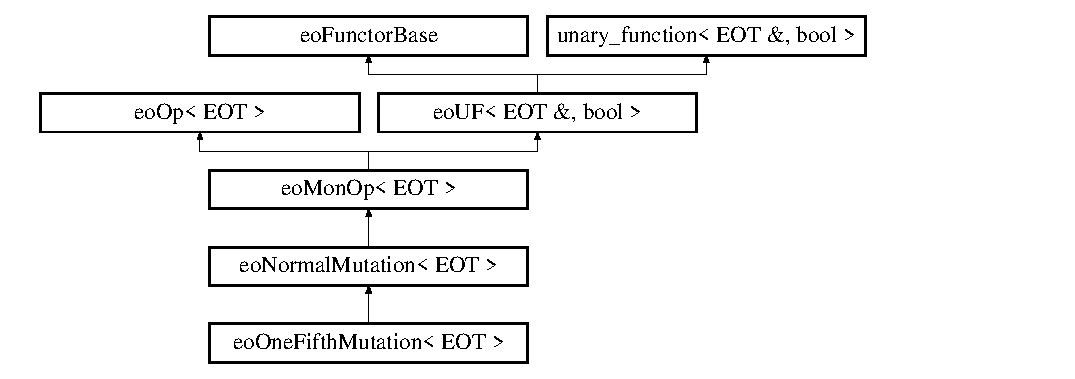
\includegraphics[height=4.64345cm]{classeo_normal_mutation}
\end{center}
\end{figure}
\subsection*{Public Member Functions}
\begin{CompactItemize}
\item 
{\bf eo\-Normal\-Mutation} (double \&\_\-sigma, const double \&\_\-p\_\-change=1.0)
\begin{CompactList}\small\item\em (Default) Constructor. \item\end{CompactList}\item 
{\bf eo\-Normal\-Mutation} ({\bf eo\-Real\-Vector\-Bounds} \&\_\-bounds, double \_\-sigma, const double \&\_\-p\_\-change=1.0)
\begin{CompactList}\small\item\em Constructor with bounds. \item\end{CompactList}\item 
virtual std::string {\bf class\-Name} () const \label{classeo_normal_mutation_a2}

\begin{CompactList}\small\item\em The class name. \item\end{CompactList}\item 
bool {\bf operator()} ({\bf EOT} \&\_\-eo)
\begin{CompactList}\small\item\em Do it! \item\end{CompactList}\item 
double \& {\bf Sigma} ()\label{classeo_normal_mutation_a4}

\begin{CompactList}\small\item\em Accessor to ref to sigma - for update and monitor. \item\end{CompactList}\end{CompactItemize}
\subsection*{Private Attributes}
\begin{CompactItemize}
\item 
double \& {\bf sigma}\label{classeo_normal_mutation_r0}

\item 
{\bf eo\-Real\-Vector\-Bounds} \& {\bf bounds}\label{classeo_normal_mutation_r1}

\item 
double {\bf p\_\-change}\label{classeo_normal_mutation_r2}

\end{CompactItemize}


\subsection{Detailed Description}
\subsubsection*{template$<$class EOT$>$ class eo\-Normal\-Mutation$<$ EOT $>$}

Simple normal mutation of a std::vector of real values. 

The st\-Dev is fixed - but it is passed ans stored as a reference, to enable dynamic mutations (see eo\-Oen\-Fith\-Mutation below).

As for the bounds, the values are here folded back into the bounds. The other possiblity would be to iterate until we fall inside the bounds - but this sometimes takes a long time!!! 



Definition at line 116 of file eo\-Normal\-Mutation.h.

\subsection{Constructor \& Destructor Documentation}
\index{eoNormalMutation@{eo\-Normal\-Mutation}!eoNormalMutation@{eoNormalMutation}}
\index{eoNormalMutation@{eoNormalMutation}!eoNormalMutation@{eo\-Normal\-Mutation}}
\subsubsection{\setlength{\rightskip}{0pt plus 5cm}template$<$class EOT$>$ {\bf eo\-Normal\-Mutation}$<$ {\bf EOT} $>$::{\bf eo\-Normal\-Mutation} (double \& {\em \_\-sigma}, const double \& {\em \_\-p\_\-change} = {\tt 1.0})\hspace{0.3cm}{\tt  [inline]}}\label{classeo_normal_mutation_a0}


(Default) Constructor. 

The bounds are initialized with the global object that says: no bounds.

\begin{Desc}
\item[Parameters:]
\begin{description}
\item[{\em \_\-sigma}]the range for uniform nutation \item[{\em \_\-p\_\-change}]the probability to change a given coordinate \end{description}
\end{Desc}


Definition at line 127 of file eo\-Normal\-Mutation.h.\index{eoNormalMutation@{eo\-Normal\-Mutation}!eoNormalMutation@{eoNormalMutation}}
\index{eoNormalMutation@{eoNormalMutation}!eoNormalMutation@{eo\-Normal\-Mutation}}
\subsubsection{\setlength{\rightskip}{0pt plus 5cm}template$<$class EOT$>$ {\bf eo\-Normal\-Mutation}$<$ {\bf EOT} $>$::{\bf eo\-Normal\-Mutation} ({\bf eo\-Real\-Vector\-Bounds} \& {\em \_\-bounds}, double {\em \_\-sigma}, const double \& {\em \_\-p\_\-change} = {\tt 1.0})\hspace{0.3cm}{\tt  [inline]}}\label{classeo_normal_mutation_a1}


Constructor with bounds. 

\begin{Desc}
\item[Parameters:]
\begin{description}
\item[{\em \_\-bounds}]an {\bf eo\-Real\-Vector\-Bounds}{\rm (p.\,\pageref{classeo_real_vector_bounds})} that contains the bounds \item[{\em \_\-sigma}]the range for uniform nutation \item[{\em \_\-p\_\-change}]the probability to change a given coordinate \end{description}
\end{Desc}


Definition at line 136 of file eo\-Normal\-Mutation.h.

\subsection{Member Function Documentation}
\index{eoNormalMutation@{eo\-Normal\-Mutation}!operator()@{operator()}}
\index{operator()@{operator()}!eoNormalMutation@{eo\-Normal\-Mutation}}
\subsubsection{\setlength{\rightskip}{0pt plus 5cm}template$<$class EOT$>$ bool {\bf eo\-Normal\-Mutation}$<$ {\bf EOT} $>$::operator() ({\bf EOT} \& {\em \_\-eo})\hspace{0.3cm}{\tt  [inline, virtual]}}\label{classeo_normal_mutation_a3}


Do it! 

\begin{Desc}
\item[Parameters:]
\begin{description}
\item[{\em \_\-eo}]The cromosome undergoing the mutation \end{description}
\end{Desc}


Implements {\bf eo\-UF$<$ EOT \&, bool $>$} {\rm (p.\,\pageref{classeo_u_f_a1})}.

Reimplemented in {\bf eo\-One\-Fifth\-Mutation$<$ EOT $>$} {\rm (p.\,\pageref{classeo_one_fifth_mutation_a2})}.

Definition at line 147 of file eo\-Normal\-Mutation.h.

References eo\-Rng::flip(), eo\-Real\-Base\-Vector\-Bounds::folds\-In\-Bounds(), and eo\-Rng::normal().

Referenced by eo\-One\-Fifth\-Mutation$<$ EOT $>$::operator()().

The documentation for this class was generated from the following file:\begin{CompactItemize}
\item 
eo\-Normal\-Mutation.h\end{CompactItemize}
